\documentclass[10pt,letterpaper]{article}

\usepackage[left=0.85in,right=0.85in,top=0.62in,bottom=0.62in,headheight=14pt]{geometry}
\usepackage{amsmath,amssymb}
\usepackage{booktabs}
\usepackage{enumitem}
\usepackage{fancyhdr}
\usepackage{graphicx}
\graphicspath{{../../}}
\usepackage{hyperref}
\usepackage{microtype}
\usepackage[section]{placeins}
\usepackage{tabularx}
\usepackage[table]{xcolor}

\makeatletter
\setlength{\@fptop}{0pt}
\makeatother

\definecolor{carma}{HTML}{1769AA}
\definecolor{ink}{HTML}{20252B}
\definecolor{muted}{HTML}{5D6670}
\definecolor{pass}{HTML}{237A45}
\definecolor{fail}{HTML}{B6423C}
\definecolor{pending}{HTML}{8A6500}
\hypersetup{colorlinks=true,linkcolor=carma,urlcolor=carma,citecolor=carma}
\urlstyle{tt}
\setlength{\parindent}{0pt}
\setlength{\parskip}{3.5pt}
\setlist{nosep,leftmargin=1.4em}
\renewcommand{\arraystretch}{1.10}
\pagestyle{fancy}
\fancyhf{}
\lhead{CARMA for GPTCache}
\rhead{Final Project Report}
\cfoot{\thepage}
\fancypagestyle{plain}{%
  \fancyhf{}
  \lhead{CARMA for GPTCache}
  \rhead{Final Project Report}
  \cfoot{\thepage}}

\newcommand{\passmark}{\textcolor{pass}{\textbf{PASS}}}
\newcommand{\failmark}{\textcolor{fail}{\textbf{FAIL}}}
\newcommand{\pendingmark}{\textcolor{pending}{\textbf{PENDING}}}
\newcommand{\invalidmark}{\textcolor{fail}{\textbf{INVALID}}}
\newcommand{\code}[1]{\texttt{#1}}
\newcommand{\reportfigure}[3]{%
  \begin{figure}[ht]
    \centering
    \includegraphics[width=\linewidth]{#1}
    \caption{#2}
    \label{#3}
  \end{figure}}

\begin{document}

\begin{titlepage}
  \centering
  \vspace*{0.55in}
  {\Huge\bfseries CARMA: Online Cluster-Adaptive Eviction for GPTCache\par}
  \vspace{0.18in}
  {\Large Cluster-Adaptive Reuse and Miss-pressure Admission\par}
  \vspace{0.42in}
  {\large Matan Goldfarb\par}
  \vspace{0.10in}
  {\normalsize Final Project Report --- August 2026\par}
  \vspace{0.45in}

  \begin{minipage}{0.90\textwidth}
  \color{ink}
  \textbf{Executive result.} I added an opt-in, CPU-only eviction policy to
  GPTCache that learns bounded semantic topics and fine-grained reuse cells online,
  adapts their quotas with decayed demand and miss pressure, and rejects weak
  one-shot admissions. The factory default and public policy interface remain
  LRU-compatible for valid existing inputs; shared normalization, validation,
  and cleanup were hardened. SQLite and FAISS deletion use vector-first
  cleanup, targeted rollback, and fail-closed reconciliation.

  On ten paired 10,000-request seeds at capacity 100, CARMA improved
  category-shift valid-hit rate by \textbf{4.885 percentage points} over the
  per-seed stronger LRU/LFU baseline (95\% paired bootstrap CI
  [4.677, 5.088], Holm-adjusted $p=0.0234$). It also passed stationary
  non-regression and synthetic weighted-savings-proxy gates. Five fresh
  SQLite/FAISS processes per
  policy showed worst ratios across seeds of 1.032$\times$ LRU for
  post-embedding cache-path p95 latency, 0.997$\times$ LRU for throughput, and
  1.043$\times$ LRU for sampled peak RSS. The reported synthetic
  ``token-saving'' result is a deterministic weighted-savings proxy, not a
  measurement of real model tokens.

  The formal full-path Gate~7 v2 attempt completed all \textbf{15/15} fresh
  children and retained \textbf{45,000} real-text ONNX requests, but its result
  is \textbf{INVALID and nonclaimable}. The preterminal auditor found seven
  evidence-contract errors, and terminalization then failed; the ledger retains
  only its canonical genesis and start events. Descriptively, 24/25 numerical
  checks pass, but seed 20261001 exceeds the CARMA--LRU p95-delta limit, so even
  counterfactually valid evidence would have produced a numerical fail.

  Two other preregistered gates \textbf{failed}. CARMA returned 30,000/30,000
  valid scan-return hits, but LFU already returned 29,998/30,000, leaving only
  +0.0067 percentage points rather than the required +5.0. Separately, strict
  QQP v2 calibration selected no threshold, so the held-out split was never
  evaluated. These negative and invalid results are preserved rather than
  converted into a favorable aggregate claim.
  \end{minipage}

  \vfill
  \begin{tabular}{@{}ll@{}}
    Software baseline & GPTCache commit \code{c59fb3a6152a4458b2a070ca183b61c4b614095f} \\
    Primary paper & SCALM, arXiv:2406.00025v1 \\
    Feature branch & \code{feature/online-cluster-aware-cache} \\
    Primary policy config & topic .70, cell .97, half-life 500, quota strength 1.0 \\
  \end{tabular}
\end{titlepage}

% Keep report navigation visible on figure-led float pages; the title page
% remains unheaded because this override is installed only after it closes.
\makeatletter
\let\ps@empty\ps@fancy
\makeatother

\section{Introduction and related work}

Semantic caches store responses under vector representations of queries and
reuse an answer when a later query is sufficiently similar. GPTCache provides
a modular open-source implementation: embeddings, vector search, similarity
evaluation, scalar/vector storage, and eviction can be configured separately
\cite{gptcache-paper}. At the selected commit, the in-memory manager offers
global LRU, LFU, FIFO, and random replacement over opaque row identifiers.
Those policies know recency or frequency, but not whether several residents
cover one redundant fine-grained reuse region or whether a miss belongs to a growing
topic.

SCALM motivates semantic structure as a cache-management signal. It analyzes
MOSS and LMSYS conversations, derives hierarchical semantic patterns, ranks
them using hit/token-saving evidence, and reports large relative gains over
GPTCache baselines \cite{scalm}. Its pattern discovery is corpus-oriented. The
question here is deliberately different:

\begin{quote}
Can a bounded policy discover useful semantic structure \emph{during} the
request stream, without offline ranking, a learned model, token cost as an
input, or a paid LLM call?
\end{quote}

Conventional cache research supplies complementary mechanisms. 2Q uses a
second-chance history to resist one-hit pollution \cite{twoq}; LRFU spans
recency and frequency through weighted history \cite{lrfu}; ARC adapts between
recency and frequency lists \cite{arc}; and TinyLFU uses approximate frequency
for admission \cite{tinylfu}. CARMA's decayed demand overlaps that adaptive
recency--frequency tradition, while its bounded repeat evidence resembles
2Q/TinyLFU admission. Its distinguishing mechanism is online semantic
organization with topic-level retention controls, not a claim that these
conventional ideas are new.

This question leads to three engineering requirements. First, answer
correctness must remain controlled by GPTCache's retrieval threshold; a policy
cluster may guide retention but may never declare a response correct. Second,
all state must remain bounded by cache capacity rather than trace length.
Third, eviction must remove scalar and vector records together so a rejected
FAISS vector cannot shadow a valid neighbor at \code{top\_k=1}.

\subsection*{Contribution and claim boundary}

The contribution is CARMA, a deterministic online policy plus backward-
compatible GPTCache integration, failure-safe cleanup, restart reconstruction,
tests, and a reproducible evaluation pipeline. The historical eight-gate audit
records Gates 1, 3, 5, 6, and 8 as pass, Gates 2 and 4 as fail, and its original
precomputed-vector Gate 7 as pending. Later real-text ONNX attempts do not
rewrite that history: formal v1 is invalid, and the complete-matrix formal v2
attempt is also invalid and nonclaimable. The internal audit is therefore
mixed (five pass, two fail, one pending); no valid formal Gate 7 pass is
claimed.

\section{Extension design}

\subsection{State and online clustering}

Each admitted entry stores a topic, a fine-grained semantic cell, insertion and
last-hit ticks, and decayed hit mass. Topics retain normalized centroids,
resident IDs, demand, and miss mass. Cells retain centroids, residents,
support, and last observation. The bounds are
$\min(64,C)$ topics and $2C$ cells for capacity $C$.

On a miss, the normalized embedding joins the highest-cosine topic above
\code{topic\_threshold}, or creates a bounded topic. The same rule assigns a
cell using \code{cell\_threshold}. Centroids use a normalized exponential
moving average. Ties always choose the lowest stable state ID. Low-support
empty cells remain temporarily as bounded ghost history, allowing a second
similar miss to challenge an incumbent even if the first candidate was
rejected.

One logical tick occurs per cache hit or inserted miss. A statistic $x$ last
updated at $t_0$ decays lazily as
\[
  x(t)=x(t_0)\,2^{-(t-t_0)/H},
\]
where $H$ is \code{demand\_half\_life}; $H=\infty$ disables decay. Lazy decay
keeps the common hit path constant-time.

\subsection{Quotas, value, and admission}

For topic $c$, recent miss pressure and quota weight are
\[
  p_c=\frac{m_c+1}{d_c+2},\qquad
  w_c=\max\{\epsilon,d_c p_c\}^{q},
\]
where $m_c$ is miss mass, $d_c$ is demand, and $q$ is
\code{quota\_strength}. Largest-remainder apportionment produces nonnegative
integer quotas that sum exactly to capacity. A resident $e$ in cell $s$ has
retention value
\[
  V_e=\frac{\operatorname{support}(s)}{\max(1,|s|)}
      +0.25\,\operatorname{hitmass}(e).
\]
The first term rewards demonstrated semantic coverage and discounts redundant
residents in the same cell.

Below capacity, every valid candidate is admitted. At capacity, a candidate is
rejected when its decayed cell support is below 1.5 or its topic quota is zero.
Otherwise it competes against the weakest eligible resident, either inside its
topic or in the most over-quota donor topic. Admission requires candidate value
at least 1.05 times victim value. Victim ties use value, last hit, insertion
age, and stable ID representation in that order.

\subsection{Complexity and intended trade-off}

Hits are $O(1)$ apart from periodic quota refresh. Miss assignment is
$O((T+S)D)$ for bounded topics $T$, cells $S$, and dimension $D$; victim
selection is $O(C)$. CARMA intentionally pays more policy CPU than LRU/LFU in
exchange for semantic coverage. It should help under phase change and
pollution, but need not dominate when a simple baseline already retains the
working set.

\section{Correctness and GPTCache integration}

Here, correctness means implementation and storage integrity; it does not
imply that semantic reuse is safe, which is evaluated separately and fails to
qualify in Section~\ref{sec:semantic-safety}. CARMA is opt-in; the factory
default and public interface remain LRU-compatible for valid existing inputs.
Shared vector normalization, validation, and cleanup were hardened. The factory
accepts \code{policy="CARMA"} and binds the storage callback internally,
avoiding a subtle failure mode in which a prebuilt custom eviction instance is
not connected to \code{SSDataManager.\_clear}. Insertions pass normalized
embeddings and persisted metadata through a backward-compatible hook.

\begin{table}[ht]
\centering
\begin{tabularx}{\linewidth}{@{}p{0.24\linewidth}X@{}}
\toprule
Invariant & Enforcement and test evidence \\
\midrule
Count/state bounds & Quotas sum to $C$; randomized sequences assert no
overflow. Topics, cells, ghosts, and custom-ID ordinals stay bounded; full
registries fail closed. \\
Scalar/vector agreement & Victims are deleted from FAISS before scalar
commit; targeted rollback preserves earlier tombstones and fails closed when
reconciliation cannot succeed. \\
Exactly-once callback & Batch victims are deduplicated and filtered against
final residents before the out-of-lock callback. \\
Malformed metadata & Missing, non-finite, zero-length, or wrong-dimensional
embeddings fail safely at full capacity. \\
Restart & Existing rows are reconstructed with a read-only scalar peek;
demand/hit mass intentionally relearn from zero. \\
Determinism & Topic, cell, quota, donor, victim, and ghost-pruning ties each
have a documented stable ordering. \\
\bottomrule
\end{tabularx}
\caption{Core safety properties exercised by unit, property, failure-path, and
SQLite/FAISS integration tests.}
\end{table}

The failure-path suite includes callback exceptions, unhashable and
representation-colliding IDs, re-admission within one batch, vector-delete
failure after scalar soft deletion, and close/reopen reconstruction. The
implementation becomes explicitly unhealthy after unrecoverable cleanup rather
than continuing with split internal/external state.

\subsection{Validation layers}

The project uses four layers: (1) focused CARMA unit/property tests; (2)
relevant upstream GPTCache eviction and SQLite/FAISS tests; (3) deterministic
CI traces with expected schemas/digests; and (4) real SQLite plus FAISS runs in
fresh child processes. Python 3.12.13 is the primary pinned target; an explicit
Python 3.8 compatibility slice protects GPTCache's older supported syntax.
No optional backend may trigger a runtime package installation during
verification.

\subsection{Restart limitation}

Resident semantic structure is reconstructed from stored embeddings, but
adaptive demand and hit mass are not persisted. They restart at zero and
relearn online. Persisting them correctly would require a versioned metadata
schema and migration rules across GPTCache backends; this is future work, not
silently simulated state.

\section{Experimental setup}

The protocol was frozen before the inferential test. Validation and test seeds
are disjoint, and test results never enter parameter selection. The 96-point
grid crosses topic thresholds $\{.70,.80,.90\}$, cell thresholds
$\{.95,.97\}$, half-lives $\{100,500,2000,\infty\}$, and quota strengths
$\{0,.5,1,2\}$. Three validation seeds and three workloads select the highest
workload-normalized valid-hit rate subject to zero synthetic false hits. The
selected configuration is (.70, .97, 500, 1.0).

\begin{table}[ht]
\centering
\begin{tabularx}{\linewidth}{@{}p{0.20\linewidth}p{0.32\linewidth}X@{}}
\toprule
Workload & Frozen construction & Purpose \\
\midrule
Stationary Zipf & 10,000 requests, exponent 1.2, 15\% one-shot & Steady skew
and non-regression. \\
Category shift & Five 2,000-request phases; 80\% demand moves & Adaptation to
new hot topics and recovery lag. \\
Pollution scan & 3,000 warm, 4,000 unique, 3,000 return & Scan resistance and
working-set recovery. \\
MOSS novel-long & Longest quartile, token-bucket stratified, 200 unique &
Exact-key LRU expected-miss control and recorded-response/token accounting;
not a CARMA overhead comparison. \\
QQP safety & Component-disjoint calibration/test split & Human-labeled semantic
precision and false-hit control. \\
\bottomrule
\end{tabularx}
\caption{Primary and safety workloads. Synthetic primary runs use capacity 100
and ten paired seeds; real system runs use five fresh processes per policy
(15 policy processes total).}
\end{table}

A hit is \emph{valid} only if the returned answer ID is allowed by the
request's ground-truth concept. False hits save zero valid tokens. Primary
metrics are valid-hit rate (VHR), hit precision, false-hit rate, opportunity
recall, and a synthetic weighted-savings proxy. In the synthetic catalog, the
per-concept weight is the deterministic formula
$16+(31t+17c+13q)\bmod 241$; it is not a tokenizer count or a SCALM token
measurement. MOSS separately records actual corpus tokens. System metrics
include request latency percentiles, throughput, CPU time, sampled RSS, and
storage invariants.

Paired deltas use 10,000-resample seed bootstraps. Confirmatory VHR comparisons
against LRU, LFU, and the per-seed stronger baseline share an exact Wilcoxon
Holm family. Capacity sweeps use the same capacity-100 traces at capacities 20,
50, 100, and 200. Ablations disable clustering, decay, admission, or
quota-aware eviction separately.

The compact synthetic catalog uses cosine 1.0 for repeated requests to the
same labeled concept, 0.96 for a deliberate distinct near-twin, 0.88 for other
distinct concepts in the same source cell, 0.72 for concepts in different
source cells of one topic, and a measured 0.00--0.12 range across topics. The
range arises because compact cell-local feature blocks are reused across
topics; it remains below the 0.70 topic threshold. At the selected 0.97 cell
threshold, no two distinct synthetic concepts share a learned CARMA cell.
Thus the primary synthetic gain cannot establish a paraphrase-cell aggregation
benefit; it mainly tests decay, admission, and retention under a controlled
geometry rather than natural-language semantic generalization.

\section{Synthetic results}

\begin{table}[ht]
\centering
\begin{tabular}{@{}lrrrc@{}}
\toprule
Workload & LRU VHR & LFU VHR & CARMA VHR & CARMA vs. stronger \\
\midrule
Stationary & 43.457\% & 47.514\% & \textbf{54.636\%} & +7.122 pp \\
Category shift & 63.376\% & 52.181\% & \textbf{68.261\%} & +4.885 pp \\
Pollution scan (whole) & 58.400\% & 59.198\% & \textbf{59.200\%} & +0.002 pp \\
Pollution return phase & 97.333\% & 99.993\% & \textbf{100.000\%} & +0.0067 pp \\
\bottomrule
\end{tabular}
\caption{Ten-seed means at capacity 100. ``Stronger'' is chosen per seed and
metric before forming paired differences.}
\end{table}

Figure~\ref{fig:vhr-deltas} summarizes the primary whole-trace comparisons.
\reportfigure{artifacts/samples/analysis/vhr-deltas.png}{Primary whole-trace VHR
difference between CARMA and the per-seed stronger LRU/LFU baseline. Error bars
are paired 95\% bootstrap intervals.}{fig:vhr-deltas}

The category-shift result passes its preregistered gate: +4.885 pp, CI
[4.677, 5.088], Holm-adjusted $p=0.0234$. Stationary performance also passes
the non-regression gate with CI lower bound +6.572 pp. The synthetic
weighted-savings-proxy deltas pass in all workloads: stationary +9.503 pp
[8.641, 10.443], shift +5.251 pp [5.009, 5.475], and pollution +0.0015 pp
[0, 0.0037]. These values use the deterministic catalog weights above, not
empirical token counts.

This is a substantive failed hypothesis, not a measurement failure. The
supplementary plot at
\path{artifacts/samples/analysis/scan-return.svg} draws the frozen +5.0 pp
line. CARMA protects the original set, but LFU protects it almost equally well:
the paired delta is +0.0067 pp, CI [0, 0.0167], Holm $p=1.0$.
In the separate exploratory 0.95-threshold hard-negative diagnostic, every
policy produced one deliberate false hit per 200 requests (0.5\% FHR), so the
CARMA--baseline false-hit difference was zero. That diagnostic tests accounting
and does not enter configuration selection or the primary threshold-0.97 claim.

\section{Sensitivity and ablations}

The labeled exploratory capacity curve is retained as
\path{artifacts/samples/analysis/capacity-curve.svg}; its fixed-trace trend is
summarized below rather than consuming another report page.

CARMA's advantage is largest when capacity is constrained and under category
shift. Averaging only for descriptive orientation across the three workloads,
its VHR is 43.49\%, 54.35\%, and 63.97\% at capacities 20, 50, and 200,
respectively, compared with LRU's 33.16\%, 46.41\%, and 60.74\%.

\begin{table}[ht]
\centering
\begin{tabular}{@{}lrrr@{}}
\toprule
Policy & Stationary & Category shift & Pollution scan \\
\midrule
CARMA & 54.636\% & \textbf{68.261\%} & 59.200\% \\
One global topic & 54.983\% & 67.874\% & 59.200\% \\
No decay & \textbf{55.108\%} & 59.980\% & 59.200\% \\
No admission & 53.025\% & 67.850\% & 55.388\% \\
No quota eviction & 54.983\% & 67.874\% & 59.200\% \\
\bottomrule
\end{tabular}
\caption{Ablation mean VHR at capacity 100. These are descriptive component
checks, not an additional confirmatory family.}
\end{table}

Decay is the clearest adaptive component: removing it loses 8.281 points on
category shift while slightly helping stationary traffic. Admission matters
most on the scan workload; disabling it loses 3.812 points. In this synthetic
geometry, replacing coarse topic clustering with one global topic changes
stationary VHR by +0.347 pp and shift VHR by -0.387 pp relative to CARMA,
while pollution is unchanged; fine-grained cell assignment remains enabled.
The no-quota result is exactly identical to the one-global-topic result despite
different topic counts. Coarse topic-clustering and quota effects are therefore
not separately identifiable here; the results do not support a standalone
claim that topic quotas preserve coverage. Decay and admission are the
strongest observed drivers.

Recovery-lag evidence is weak: CARMA averages 1,808 requests versus the
2,000-request censoring limit for both baselines. Yet 31/40 CARMA and all 40
baseline transitions are censored; exploratory exact Wilcoxon $p=0.0625$.

\section{Real-system, MOSS, and semantic-safety evidence}

The system benchmark uses the actual GPTCache \code{SSDataManager}, SQLite,
and FAISS path, but replays precomputed vectors from the controlled synthetic
catalog rather than running \code{paraphrase-albert-onnx}. Each policy runs in
a fresh process on the same 3,000-request pollution trace, with immediate
physical deletion and a final round-trip check of every active vector. Across
five seeds, every run has zero false hits, zero stale candidates, and equal
final scalar/vector counts.

Figure~\ref{fig:system} separates policy-only work from post-embedding cache-path
cost.
\reportfigure{artifacts/samples/analysis/latency-resources.png}{Real
SQLite/FAISS measurements using precomputed synthetic vectors. Bars are
five-seed means and circles are individual fresh-process runs. Policy-only
overhead is shown separately from post-embedding cache-path request cost;
embedding generation is excluded.}{fig:system}
\FloatBarrier

\begin{table}[ht]
\centering
\begin{tabular}{@{}lrrrr@{}}
\toprule
Policy & Mean & p50 & p95 & p99 \\
\midrule
LRU & 1.804 ms & 1.032 ms & 3.511 ms & 4.602 ms \\
LFU & 1.724 ms & 0.953 ms & 3.433 ms & 4.181 ms \\
CARMA & 1.723 ms & 0.875 ms & 3.469 ms & 3.952 ms \\
\bottomrule
\end{tabular}
\caption{Five-seed means of each fresh process's request-latency summaries.
The measured scope is the post-embedding cache path using precomputed vectors.}
\end{table}

CARMA adds roughly 354 $\mu$s to policy-only p95, reflecting bounded cosine
assignment and victim selection. Post-embedding cache-path p95 nevertheless
ranges from
0.936$\times$ to 1.032$\times$ LRU because policies create different hit,
admission, and storage-cleanup mixes. The worst ratio across seeds is
0.997$\times$ LRU for throughput and 1.043$\times$ LRU (+4.8 MiB) for sampled
peak RSS. Mean one-core CPU utilization is 96.9\% for CARMA versus 94.1\% for
LRU. GPU use is not applicable to this CPU-only path, and macOS did not expose
portable process I/O byte counters. Every seed satisfies the individual
numerical checks; the historical Gate 7 entry remains pending because its
contract omitted an across-seed aggregation rule and specified an ONNX
integration embedding that this run did not use.

Only each run's mean and quantiles were retained; individual request-latency
samples were not retained in the integration artifacts. Figure~\ref{fig:system}
therefore shows the
cross-seed distribution of p95 summaries, not a reconstructable per-request
CDF. This is an artifact-granularity limitation despite collecting the frozen
mean, p50, p95, and p99 metrics in process. The later v2 attempt does retain
per-request samples; Figure~\ref{fig:gate7-v2-latency} shows them only as an
explicitly invalid, descriptive supplement.

\subsection{Formal full-path ONNX v2: complete matrix, invalid evidence}

Gate 7 has three distinct generations and none is a formal pass
(Table~\ref{tab:gate7-lineage}). The historical integration study used real
SQLite/FAISS but precomputed synthetic vectors, so it remains diagnostic and
pending. Formal v1 used real text and ONNX, but stopped after its first child
when its original protocol treated a labeled-negative semantic return as
structural corruption; that attempt remains invalid. Formal v2 prospectively
separated systems validity from semantic safety and ran the complete matrix,
but failed its own evidence and terminalization contract.

\begin{table}[ht]
\centering
\begin{tabularx}{\linewidth}{@{}p{0.16\linewidth}p{0.30\linewidth}p{0.15\linewidth}X@{}}
\toprule
Generation & Measured path & Status & Claim boundary \\
\midrule
Historical & SQLite/FAISS with precomputed synthetic vectors & \pendingmark &
Post-embedding diagnostics only; no frozen full-path ONNX adjudication. \\
Formal v1 & Real QQP text, ONNX, one completed CARMA child & \invalidmark &
Incomplete matrix and structurally conflated semantic failure. \\
Formal v2 & Real QQP text, ONNX, all 15 fresh children & \invalidmark &
Complete data, but seven preterminal errors and no terminal ledger event. \\
\bottomrule
\end{tabularx}
\caption{Gate 7 lineage. Each generation is preserved under its own protocol;
later evidence does not repair or reinterpret an earlier attempt.}
\label{tab:gate7-lineage}
\end{table}

The v2 runner measured the complete \code{gptcache.adapter.adapter.adapt} path:
real calibration text, checksum-pinned 768-dimensional ALBERT ONNX embedding,
similarity, SQLite, FAISS, eviction, recorded miss response, and response
return. LRU, LFU, and CARMA used an identical 3,000-request trace for each of
five seeds, capacity 100, fresh child processes and storage, and the frozen
counterbalanced order. All 15 children exited zero and produced 45,000 request
rows with mutually exclusive stage timings plus external resource samples.

The retained attempt is under
\path{artifacts/gate7-v2-onnx-attempts/}, in
\path{attempt-20260827T131736Z-1784}. Its immutable preterminal report uses
schema \code{carma-gate7-adjudication-v2}. It records phase
\code{preterminal}, status \code{invalid}, \code{claimable=false}, and seven
errors:
one dependency-attestation error conflates lexical and resolved Python
identities; each of five warm-up declarations includes an extra \code{rows}
field instead of exactly \{\code{sha256}, \code{bytes}\}; and seed 20261003
LRU has a 202,142,875-ns resource-sampling gap, 2,142,875 ns beyond the frozen
200,000,000-ns limit. Terminalization then rejected the manifest's auditor
identity \{\code{bytes}, \code{sha256}\} because the preterminal report records
\{\code{path}, \code{bytes}, \code{sha256}\}. The wrapper exited 4. The root
ledger therefore contains only canonical \code{PROTOCOL\_GENESIS} and
\code{START} rows---no \code{TERMINAL}---and no ordinary
\code{gate7-adjudication.json} exists.

The numerical reconstruction is descriptive only. Twenty-four of 25 frozen
per-seed systems checks pass. The sole failure is seed 20261001 p95 latency
delta: CARMA is 470,385,875 ns versus LRU's 444,155,750 ns, a 26,230,125-ns
increase against a 500,000-ns maximum. Seeds 20261002--20261005 pass all five
checks. Because the rule requires every check for every seed, a counterfactual
structurally valid version of these same measurements would numerically
\emph{fail}, not pass.

Figure~\ref{fig:gate7-v2-latency} pools exactly 3,000 requests from each of
five seeds for each policy. The left panel shows full-request latency on a
linear axis; the right isolates the post-embedding path on a labeled log axis.
The much smaller post-embedding scale makes clear that ONNX embedding dominates
full-path latency, while the policy curves still have different tails. These
curves are useful for diagnosing where overhead occurs, but the invalid ledger
means they cannot rank policies formally. The exact 5-by-5 frozen-check matrix
remains available as a supplementary figure in the curated analysis package.

\begin{figure}[ht]
\centering
  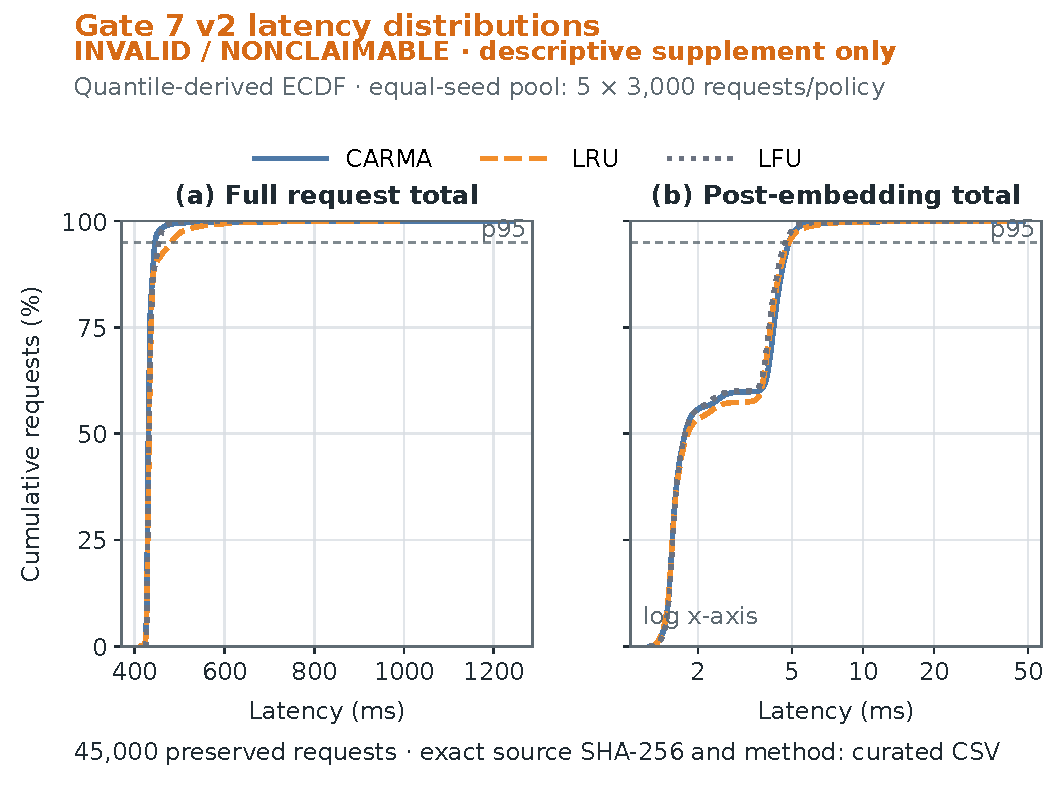
\includegraphics[width=\linewidth]{artifacts/samples/analysis/gate7-v2-invalid/gate7-v2-latency-distributions.pdf}
\caption{Descriptive Gate 7 v2 full-request and post-embedding latency
distributions for 45,000 preserved requests. Curves are quantile-derived ECDF
approximations from an equal-seed pool. The source attempt is \textbf{INVALID}
and nonclaimable; the figure is not a Gate 7 verdict.}
\label{fig:gate7-v2-latency}
\end{figure}

Semantic safety is reported on a separate axis. Across 25,405 cache hits,
25,400 are same-component, three are direct-negative, and two are unlabeled
cross-component; no hit is component-derived-negative or unresolved. The 15
run statuses are three \code{FAIL}, two \code{PENDING\_INDETERMINATE}, and ten
\code{PASS\_OBSERVED}. Thus the aggregate semantic guardrail is \failmark{},
independently of the invalid systems evidence and independently of Gate 2.
\FloatBarrier

\subsection{Pinned MOSS exact-key recorded-response replay}

The CC-BY-4.0 MOSS archive \cite{moss-source} is fixed by repository revision
and SHA-256. A full
streaming CRC-verified pass covers 301,332 source conversations and 823,634
actual turns, then retains the lowest stable-hash 2,048-turn sample. The
200-request longest-quartile trace contains 557,243 context, prompt, and answer
tokens. The replay uses an exact-key LRU cache. All requests are unique by
design, so all 200 are misses, every recorded MOSS answer is delivered, and
live model calls, cache hits, and false hits are all zero. Two runs produce
byte-identical manifests, pool, requests, and CSV. This validates source and
token accounting, but the lecturer's novel-long overhead criterion is only
partial: this run neither compares CARMA/LRU/LFU semantic policies nor measures
valid end-to-end long-prompt CARMA overhead.

The real archive also exposed 30,000 rows with \code{conversation\_id=-1} and
2,727 declared-turn-count mismatches. Before producing a result, the parser was
amended to hash canonical rows for negative sentinel IDs and to treat
contiguous chat keys as authoritative while retaining both declared and actual
counts. The final manifest records these anomalies and preserves the separate
prepare manifest.

\subsection{Held-out QQP safety}\label{sec:semantic-safety}

The component-disjoint calibration set contained 7,729 pairs: 5,652 positives
and 2,077 negatives. None of the 20 frozen thresholds from 0.80 through 0.99
met the strict v2 selection rule. At threshold 0.96, precision is
0.97574893 and its one-sided 95\% Wilson lower bound is 0.96420782; the
false-hit rate is 0.00219951 and its one-sided Wilson upper bound is
0.00326719. Its Wilson precision lower bound is below the
calibration-selection requirement of 0.99, and no other grid point qualifies,
so the selected threshold is null. The separate downstream Gate 2 targets---
held-out point precision at least 0.99, Wilson lower bound at least 0.98, and
the CARMA false-hit-rate delta bound---were therefore never reached or
evaluated. The protocol did not resolve held-out endpoints: all 56,963
held-out rows remain unevaluated, and no held-out precision or false-hit claim
is made. Gate 2 is therefore \failmark{} regardless of the separate Gate 7
trace observations.

\begin{table}[ht]
\centering
\begin{tabularx}{\linewidth}{@{}p{0.07\linewidth}p{0.14\linewidth}X@{}}
\toprule
Gate & Status & Historical eight-gate adjudication \\
\midrule
1 & \passmark & Exact-source host verifier passed; integration integrity
failures are zero. \\
2 & \failmark & No QQP calibration threshold met the precision prerequisite;
held-out evaluation was not run. \\
3 & \passmark & Shift VHR +4.885 pp; CI [4.677, 5.088]; Holm $p=.0234$. \\
4 & \failmark & Return VHR +0.0067 pp versus required +5.0 pp. \\
5 & \passmark & Stationary VHR delta CI lower bound +6.572 pp. \\
6 & \passmark & Synthetic weighted-savings-proxy delta CI lower bound meets
every workload limit. \\
7 & \pendingmark & The historical precomputed-vector study is diagnostic only;
formal ONNX v1 and v2 are separately \textbf{INVALID}, not replacements for
this row. \\
8 & \passmark & Two fresh network-isolated \code{linux/amd64} runs produced
byte-identical benchmark artifacts and normalized logs. \\
\bottomrule
\end{tabularx}
\caption{Historical success-gate table. Gates 2 and 4 remain failed; the
original Gate 7 remains pending, while Table~\ref{tab:gate7-lineage} records
the later formal v1 and v2 invalid attempts without rewriting this audit.}
\end{table}

\section{Discussion, protocol audit, and limitations}

\subsection{What the experiments establish}

CARMA's strongest evidence is phase adaptation: decay prevents obsolete
lifetime popularity from dominating after a topic shift, and admission
protects scan performance. The ablations do not separately identify a benefit
from clustering or quotas, so they cannot support a causal quota-coverage
claim. The implementation cost is measurable in policy-only latency. All
historical precomputed-vector seeds stay inside their diagnostic limits, but
formal v2 has one descriptive p95-delta failure and is structurally invalid.
The evidence therefore supports an adaptive-policy contribution driven most
clearly by decay and admission, not a formal Gate 7 performance pass.

The scan gate explains why raw perfection is not enough. CARMA achieves 100\%
return VHR, but the correct comparator is the stronger paired baseline, not
LRU alone. LFU is already 99.993\%; the prespecified five-point margin is
impossible to claim from this trace. A future scan workload should make the hot
set large enough, or interleave enough recurrent cold items, to distinguish
coverage policies without changing the gate after observation.

\subsection{Post-execution protocol conformance}

The historical full bundle's hashes, seed pairing, selected configuration, 480 aggregate
rows, bootstraps, Wilcoxon tests, and Holm adjustment were independently
recomputed exactly. That audit also found six deviations that this report does
not hide:

\begin{enumerate}
  \item the historical full bundle contains summary CSVs/metadata but not the
  promised per-request and process-resource JSONL, limiting reconstruction of
  individual phase events from that bundle alone;
  \item synthetic policy execution order is fixed rather than randomized;
  state is isolated and timing is disabled, so this is unlikely to bias VHR;
  \item synthetic false-hit intervals are seed bootstraps, not Wilson bounds;
  they must not be cited as the substantive semantic-safety interval; and
  \item the preregistered scale sweep and secondary negative/ceiling controls
  were not run. Capacity sweeps and the four component ablations were run; and
  \item the integration runs used precomputed 2,982-dimensional synthetic
  vectors rather than the frozen ONNX embedding, so their timing covers only
  the post-embedding cache path and Gate 7 remains diagnostic; and
  \item the QQP implementation computed held-out cosine similarities
  transiently before the calibration abort, although it never selected a
  threshold, classified or aggregated held-out labels, exposed held-out
  metrics, or wrote those similarities.
\end{enumerate}

The exact historical result remains tied to clean commit
\code{28129f0b9785232827e741c0e2ff2bb96cc19423}; later tooling changes cannot
retroactively alter its status. A separate deviation ledger documents impact
and future-run remediation.

The final correctness and reproducibility evidence is tied to exact source
commit:
\newline\code{557c6ac0578cb6b77c5ae51595b49abdc0407e10}.
The clean host and both containers used the same 527-file Git archive,
SHA-256:
\newline\code{51aea800e364c1d52bed566f48c4c49c1836d0d6a0b40b3bb8203867c14b58b4}.
The report and curated evidence are the only changes in its single permitted
direct packaging child. Gate 7 v2 is separately bound to that clean source,
but it inherits no pass from the host/container reproducibility gate: its
complete data and seven preterminal findings remain frozen under an unmatched
\code{START}, and neither manifest nor ledger may be repaired in place.

\subsection{External validity}

Synthetic vectors isolate eviction behavior but are not natural language.
QQP calibration probes pairwise semantic matching; its component-disjoint
held-out split was not evaluated, and neither represents conversational
distribution shift. MOSS is an exact-key recorded-response negative control
rather than a CARMA semantic-policy or long-prompt overhead comparison.
Historical system timing
excludes embedding; v2 includes real ONNX embedding but is invalid evidence.
Both use one Apple-arm64 machine, five seeds, capacity 100, and SQLite/FAISS.
Restart loses adaptive counters. These boundaries limit generalization but
make each retained claim traceable.

\section{Conclusion and future work}

This project delivers a cleanly factored GPTCache feature branch, an online
cluster-aware policy, robust cross-store deletion, focused and upstream tests,
frozen paired experiments, real backend measurements, pinned natural-data
checks, deterministic analysis, container/CI definitions, and an auditable
report. A 5,180,400-evaluation final-source replay reproduced all four published
synthetic CSV summaries byte-for-byte. The central hypothesis is only partly
supported: CARMA is compelling
under category shift and passes stationary VHR non-regression, but semantic
safety fails at QQP calibration and its preregistered scan advantage over the
strongest baseline fails. The full-path Gate 7 v2 matrix is complete, yet the
attempt is invalid and nonclaimable; its descriptive measurements also contain
one decisive p95-delta failure.

The next formal run must use a \emph{new} protocol version, contract,
experiment ID, formal root, ledger, and annotated source tag, followed by a
fresh complete 5$\times$3 matrix. V2 must never be repaired or selectively
rerun. Before that new registration, identities should be canonicalized;
lexical and resolved Python executables must be separate fields; the warm-up
artifact schema and auditor must agree exactly; the resource sampler needs a
deadline-aware cadence margin; and lifecycle tests must cover preterminal
identity transfer, bootstrap completion, terminal append, and ordinary audit.
Performance work should optimize CARMA p95 first, because seed 20261001 misses
the absolute latency-delta bound by 25.73 ms even though its ratio passes.
Public PR \href{https://github.com/zilliztech/GPTCache/pull/696}{zilliztech/GPTCache\#696}
targets \code{dev}; it is mergeable and DCO-passing, but no maintainer has
reviewed or adopted it. The exceptional adopted-PR route therefore remains an
unmet external criterion.

\section*{Lecturer-criterion audit}

\begin{tabularx}{\linewidth}{@{}p{0.18\linewidth}p{0.15\linewidth}X@{}}
\toprule
Criterion & Status & Evidence \\
\midrule
Correctness (40\%) & Implementation \passmark; semantic \failmark & The
exact-source host verifier passed 8 upstream plus 2 SQLite/FAISS tests
(1 optional deselected) and 453 project tests (4 skipped); real integration
integrity failures are zero. QQP calibration selected no qualifying threshold,
so semantic reuse safety is not established. \\
Reproducibility (30\%) & \passmark & Exact pins and one source archive produced
matching host plus two fresh network-isolated container benchmark artifacts;
evidence is checksum-linked; a final-source replay reproduced all four
synthetic summaries byte-for-byte. \\
Performance (15\%) & Mixed & Gates 3, 5, 6 pass; Gates 2 and 4 fail; each
historical system seed meets its diagnostics, while formal Gate 7 v1 and v2
are invalid and v2 descriptively fails one of 25 systems checks. \\
Clarity (15\%) & Complete with caveat & Baseline rationale, policy/protocol
docs, labeled figures, limitations, and this report are complete; the sealed
README's old formal-run command is superseded by the handoff. \\
\bottomrule
\end{tabularx}

\section*{Appendix: Artifact map}

Code and tests are under \path{gptcache/manager/} and \path{tests/}; experiments
and wrappers are under \path{benchmarks/carma/} and \path{scripts/}; course docs
are under \path{docs/project/}; and curated checksummed evidence is under
\path{artifacts/samples/}. The authoritative v2 root under
\path{artifacts/gate7-v2-onnx-attempts/} is local and ignored, not shipped in a
fresh clone. Environment/CI definitions are \path{Dockerfile.project},
\path{requirements-*.lock}, and \path{.github/workflows/carma-ci.yml}.

\begingroup
\setlength{\parskip}{0pt}
\setlength{\itemsep}{0pt}
\setlength{\parsep}{0pt}
\begin{thebibliography}{9}
\bibitem{gptcache-paper}
Bang Fu and Di Feng. ``GPTCache: An Open-Source Semantic Cache for LLM Applications
Enabling Faster Answers and Cost Savings.'' \emph{NLP-OSS 2023}, pp. 212--218.
\href{https://doi.org/10.18653/v1/2023.nlposs-1.24}{doi:10.18653/v1/2023.nlposs-1.24}.

\bibitem{scalm}
J. Li, C. Xu, F. Wang, I. M. von Riedemann, C. Zhang, and J. Liu.
``SCALM: Towards Semantic Caching for Automated Chat Services with Large
Language Models.'' arXiv:2406.00025v1, 2024.
\href{https://arxiv.org/abs/2406.00025}{arxiv.org/abs/2406.00025}.

\bibitem{twoq}
Theodore Johnson and Dennis Shasha. ``2Q: A Low Overhead High Performance
Buffer Management Replacement Algorithm.'' \emph{VLDB 1994}, pp. 439--450.
\href{https://www.vldb.org/conf/1994/P439.PDF}{vldb.org/conf/1994/P439.PDF}.

\bibitem{lrfu}
Donghee Lee et al. ``LRFU: A Spectrum of Policies that Subsumes the Least
Recently Used and Least Frequently Used Policies.'' \emph{IEEE Transactions
on Computers} 50(12), 2001, pp. 1352--1361.
\href{https://doi.org/10.1109/TC.2001.970573}{doi:10.1109/TC.2001.970573}.

\bibitem{arc}
Nimrod Megiddo and Dharmendra S. Modha. ``ARC: A Self-Tuning, Low Overhead
Replacement Cache.'' \emph{FAST 2003}.
\href{https://www.usenix.org/conference/fast-03/presentation/arc-self-tuning-low-overhead-replacement-cache}{USENIX proceedings page}.

\bibitem{tinylfu}
Gil Einziger, Roy Friedman, and Ben Manes. ``TinyLFU: A Highly Efficient Cache
Admission Policy.'' \emph{ACM Transactions on Storage} 13(4), Article 35,
2017. \href{https://doi.org/10.1145/3149371}{doi:10.1145/3149371}.

\bibitem{moss-source}
OpenMOSS Team. ``moss-003-sft-data,'' revision
\code{42e216d3e3fb331c18d5fa6e7cb4f1c53eef24a4}, CC-BY-4.0.
\href{https://huggingface.co/datasets/OpenMOSS-Team/moss-003-sft-data}{dataset}.

\end{thebibliography}
\endgroup

\end{document}
